\chapter{INTRODUÇÃO}\label{chp:INTRODUCAO}

Parte inicial do texto, na qual devem constar o tema e a delimitação do assunto tratado, objetivos da pesquisa e outros elementos necessários para situar o tema do trabalho. Após o início de uma seção, recomenda-se a inserção de um texto ou, no mínimo, uma nota explicativa sobre a seção iniciada. Evitar, por exemplo, figura \ref{fig:WhatNotToDo}:

\begin{figure}[htb]
	\centering
	\caption{Exemplo do que não é recomendado.}
	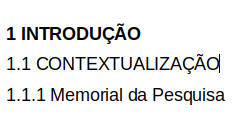
\includegraphics[scale=0.6]{imagens/what-not-to-do.png} 
	\newline \footnotesize \textbf{Fonte: Autoria própria.}
	\label{fig:WhatNotToDo}
\end{figure}

\section{OBJETIVOS}\label{sec:OBJETIVOS}
Expõem-se a seguir os objetivos geral e específicos que se pretende atingir com o trabalho . Ver mais exemplos no Anexo 1. 

\subsection{Geral}\label{sec:Geral}
Desenvolver um sistema de Internet of Things (IoT) automatizado que controle a entrada e saída de pessoas em áreas de acesso restrito, identifique suas funções institucionais por meio da tecnologia RFID, e registre o acesso via portas com trava ou catraca.


\subsection{Específicos}\label{sec:Especificos}
\begin{enumerate}
	\item Estudar conceitos básicos relativos a controle de acesso orientado a contextos; 
	
	\item Fazer uma proposta inicial de ambiente;
	
	\item Implementar um protótipo;
	
	\item Desenvolver um módulo Web para controle por parte do administrador, que permita monitorar os registros e gerenciar permissões
\end{enumerate}


\section{CONTRIBUIÇÕES DO TRABALHO}\label{sec:CONTRIBUICOES}
Explicitar as contribuições do trabalho para a sociedade, ou seja, sua pertinência. Por exemplo, no desenvolvimento de um sistema de controle com IoT, a contribuição é o ganho que um sistema desses pode trazer à área de organização escolar, uma vez que automatiza por completo as tarefas, junto com uso eficiente de TFID aliado a um sistema de controle funcional pela Web. Com essas características, o sistema apresenta melhorias em relação ao controle tradicional feito nesses ambientes e supera outras abordagens que não consideram as automatizações aqui propostas. [verificar enumeração]


\section{JUSTIFICATIVA}\label{sec:JUSTIFICATIVA}
A justificativa refere-se a por que é importante e válida a realização do trabalho. Trata-se de convencer o leitor de que o trabalho de pesquisa  apresenta contribuições específicas para a Ciência da Computação. Deve exaltar a importância da pesquisa e a relação de outras pesquisas sobre os mesmos assuntos. [adaptar texto para diferenciar do \ref{sec:CONTRIBUICOES}, colocar exemplo aqui e diretriz no comentário].


\section{DELIMITAÇÕES DO TRABALHO}\label{sec:DELIMITACOES}
Identificar e justificar aqui as delimitações do trabalho em relação a sua construção e objetivos a ser alcançados. Limitações podem estar presentes na: forma como os experimentos foram conduzidos, por falta de, por exemplo, equipamento específico, software ou recursos em geral; forma como a metodologia foi estabelecida, ignorando alguma etapa que por ventura existe, mas não será abordada devido ao viés do trabalho; ou em características gerais do trabalho, em que alguma limitação foi imposta para adequação à construção do trabalho e satisfação dos objetivos principais. [escopo, exemplo]
